% !TEX root = ../main.tex
\section{Q15: Nyttefunksjoner -- integritet vs.\ indkomst, risiko vs.\ forventet verdi}\label{q:15}

\begin{quote}
\emph{Med udgangspunkt i pensums anvendelse af økonomisk teoris nyttebegreb samt nyttefunktioner, bedes du redegøre for modellen, der illustrerer hvordan designet af kompensationsplaner kan påvirke medarbejderes valg af ``goder'' (f.eks.\ integritet versus indkomst). I forlængelse heraf bedes ligeledes skitseret modellen, der viser hvorledes indifferenskurver kan håndtere og afspejle sammenhængen mellem risiko og forventet værdi.}
\end{quote}

\subsection*{Svar (kort)}
Spørsmålet besvares med to nyttemodeller fra BSZ kap.\ 2. \textbf{Modell 1 (integrity vs.\ income):} Kompensasjonsdesignet endrer agentens budsjettbetingelse mellom integritet og indkomst; et aggressivt insentivsystem roterer budsjettlinjen slik at gevinsten ved å ofre integritet øker, og agenten velger lavere integritet -- selv uten endring i preferanser. \textbf{Modell 2 (risk vs.\ expected value):} Indifferenskurver i $(\sigma, E[W])$-rommet viser at en risikoavers agent krever høyere forventet lønn for å akseptere mer risiko; helningen bestemmes av risikoaversjons\-parameteren $r$, og risikopremien er avstanden mellom forventet verdi og certainty equivalent. [SLIDE]

\subsection*{Relevante teorier (kort)}

\paragraph{\thref{integrity-vs-income-model}{Modell 1: Integrity vs.\ Income}\quad\SThree}
Standard nytteteori overført til godsrommet (integritet, indkomst). Indifferenskurver er konvekse mot origo. Budsjettlinjen defineres av kompensasjonsplanen: aggressivt insentiv (høy $\beta$ på lett målbare resultater uten kvalitetssjekk) roterer budsjettlinjen utover og øker payoffen av uetisk atferd. Tangentpunktet skifter fra punkt $A$ (høy integritet) til $B$ (lav integritet, høy inntekt). Nøkkelinnsikt: kompensasjonsdesign påvirker etisk atferd uten å endre preferanser -- det er \emph{systemet}, ikke personen, som er feil. [SLIDE]

\paragraph{\thref{risk-expected-value-model}{Modell 2: Risk--Expected Value}\quad\SThree}
CARA-nytte gir indifferenskurver $E[W] = \bar{U} + \tfrac{r}{2}\sigma_W^2$ -- stigende og konvekse oppover i $(\sigma_W, E[W])$-rommet. Risikoavers agent ($r>0$): bratte kurver. Risikonøytral ($r=0$): horisontale. Certainty equivalent $CE$ = skjæring med $y$-aksen. Risikopremie $RP = E[W] - CE = \tfrac{r}{2}\beta^2\sigma^2$. Modellen visualiserer \thref{risk-sharing}{risikodeling}: prinsipalen tilbyr en kontrakt (punkt i rommet); agenten aksepterer bare hvis den når minst \thref{reservation-utility}{reservation utility}. [SLIDE]

\paragraph{\thref{incentive-coefficient}{Incentive coefficient $\beta$}\quad\SThree}
$\beta$ kobler de to modellene: i modell 1 driver $\beta$ rotasjonen av budsjettlinjen (høy $\beta$ øker fristelsen til uetisk atferd). I modell 2 driver $\beta$ risikoen $\sigma_W = \beta\sigma$ og dermed risikopremien. Samme designparameter, to konsekvenser -- understreker at insentivdesign er en \emph{trade-off} mellom innsatsgevinst, risikokostnad \emph{og} etisk atferd. [SLIDE]

\subsection*{Grafisk modell 1 -- Integrity vs.\ Income}

\begin{figure}[h]
\centering
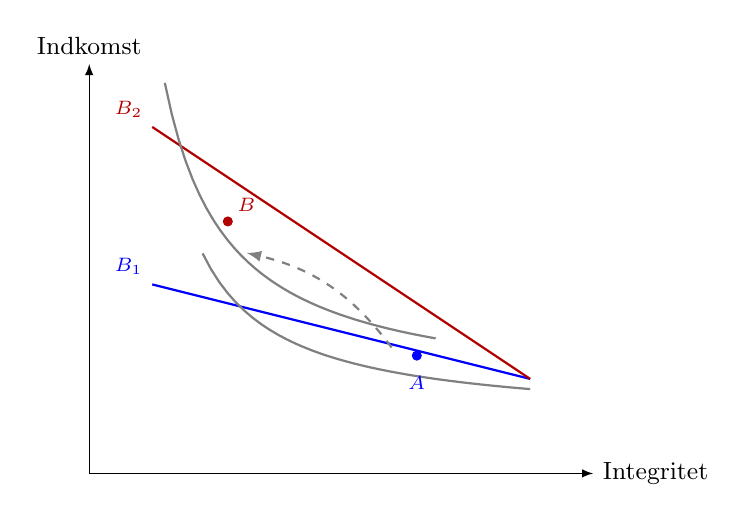
\begin{tikzpicture}[>=latex, scale=0.8, every node/.style={font=\small}]
  \draw[->] (0,0) -- (8,0) node[right] {Integritet};
  \draw[->] (0,0) -- (0,6.5) node[above] {Indkomst};
  % B1 moderat
  \draw[thick, blue] (1.0,3.0) -- (7.0,1.5);
  \node[blue, above left, font=\scriptsize] at (1.0,3.0) {$B_1$};
  % B2 aggressiv
  \draw[thick, red!70!black] (1.0,5.5) -- (7.0,1.5);
  \node[red!70!black, above left, font=\scriptsize] at (1.0,5.5) {$B_2$};
  % Indifferenskurver
  \draw[thick, gray, domain=1.8:7.0, samples=40]
    plot (\x, {3.5/(\x-0.5) + 0.8});
  \draw[thick, gray, domain=1.2:5.5, samples=40]
    plot (\x, {5.0/(\x-0.2) + 1.2});
  % Punkt A
  \filldraw[blue] (5.2,1.87) circle (2pt);
  \node[below, blue, font=\bfseries\scriptsize] at (5.2,1.7) {$A$};
  % Punkt B
  \filldraw[red!70!black] (2.2,4.0) circle (2pt);
  \node[above right, red!70!black, font=\bfseries\scriptsize] at (2.2,4.0) {$B$};
  \draw[->, thick, dashed, gray] (4.8,2.0) to[bend right=20] (2.5,3.5);
\end{tikzpicture}
\caption{\textbf{Integrity vs.\ Income.} $B_1$ (moderat insentiv): optimum $A$ med høy integritet. $B_2$ (aggressivt insentiv): optimum $B$ med lav integritet, høy inntekt. Kompensasjonsdesignet endrer atferd uten å endre preferanser. [SLIDE -- BSZ kap.\ 2]}
\end{figure}

\subsection*{Grafisk modell 2 -- Risk vs.\ Expected Value}

\begin{figure}[h]
\centering
\begin{tikzpicture}[>=latex, scale=0.8, every node/.style={font=\small}]
  \draw[->] (0,0) -- (8,0) node[right] {$\sigma_W$ (risiko)};
  \draw[->] (0,0) -- (0,7) node[above] {$E[W]$};
  % Risikoavers
  \draw[thick, blue, domain=0:5.5, samples=40]
    plot (\x, {1.5 + 0.15*\x*\x});
  \node[blue, right, font=\scriptsize] at (5.5,6.0) {risikoavers ($r>0$)};
  \draw[thick, blue, dashed, domain=0:4.5, samples=40]
    plot (\x, {2.5 + 0.15*\x*\x});
  % Risikonøytral
  \draw[thick, green!50!black] (0,3.0) -- (7.0,3.0);
  \node[green!50!black, right, font=\scriptsize] at (7.0,3.0) {risikonøytral ($r=0$)};
  % CE og RP
  \node[left, font=\scriptsize] at (0,1.5) {$CE$};
  \filldraw[blue] (3.5,3.34) circle (1.5pt);
  \node[above left, font=\bfseries\scriptsize, blue] at (3.5,3.34) {$A$};
  \draw[dashed] (3.5,0) -- (3.5,3.34);
  \draw[dashed] (0,3.34) -- (3.5,3.34);
  \node[left, font=\scriptsize] at (0,3.34) {$E[W]_A$};
  \draw[decorate, decoration={brace, amplitude=4pt, mirror}, red!70!black] (-0.3,1.5) -- (-0.3,3.34);
  \node[left, font=\scriptsize, red!70!black] at (-0.6,2.42) {$RP$};
  \node[below, font=\scriptsize] at (3.5,0) {$\sigma_A$};
\end{tikzpicture}
\caption{\textbf{Risk--Expected Value.} Risikoavers agent (blå): stigende, konvekse indifferenskurver. $CE$ = certainty equivalent (skjæring $y$-akse). $RP = E[W]_A - CE = \tfrac{r}{2}\beta^2\sigma^2$. Risikonøytral (grønn): flat -- ingen risikopremie. [SLIDE -- BSZ kap.\ 2/15]}
\end{figure}

\subsection*{Real-world eksempler}

\textbf{Eks.~1 -- Wells Fargo (2016) -- integrity vs.\ income i praksis.}\quad [EKS]
Wells Fargos aggressive cross-sell-kvoter (høy $\beta$ på antall solgte produkter) roterte budsjettlinjen i integrity-income-rommet. Ansatte valgte punkt $B$: 3{,}5 mill.\ falske kontoer åpnet. Etter skandalen (\$185M bot, CEO trådte av) ble $\beta$ redusert og kvalitative mål innført -- budsjettlinjen rotert tilbake mot integritet. Modell 1 forklarer mekanismen presist: det var systemet, ikke personene, som var feil.

\textbf{Eks.~2 -- Equinor-ansatte og aksjespareprogram, sammenligning.}\quad [EKS]
Equinor tilbyr aksjeprogram med rabatt: ansatte velger frivillig mellom lav-risiko (fastlønn, 100\%) og høy-risiko (fastlønn + aksjer, usikkert). Konservative ingeniører med høy boliggjeld velger lite eksponering (bratte indifferenskurver, høy $r$). Risikotolerante seniorledere velger mer aksjer (flate kurver, lav $r$). Modell 2 forklarer seleksjonsmønsteret. Sammenligningen med Wells Fargo: begge handler om kompensasjonsdesignets effekt på atferd -- Wells Fargo om etisk dimensjon (modell 1), Equinor om risiko-dimensjon (modell 2). Samme nytteteori, to ulike godsrom.

\subsection*{Kobling til Mærsk Power-to-X}
\textbf{Modell 1:} PtX-prosjektledere kan fristes til å oppblåse prognoser og underkommunisere risiko hvis bonusen er knyttet til prosjektgodkjenning -- budsjettlinjen premierer ``lav integritet'' (overoptimistiske estimater). Løsning: claw-back-klausuler og subjektiv evaluering som bevarer integritet-insentiv. \textbf{Modell 2:} PtX har svært stor $\sigma$ (teknologirisiko, reguleringsrisiko, markedsrisiko). Risikoaverse ledere krever høy $E[W]$ for å akseptere stillingen -- synlig i PtX-divisjonens lønnsstruktur: høy grunnlønn + moderat $\beta$ på milestones (jf.\ \thref{informativeness-principle}{informativeness}). [CASE]

\subsection*{Fallgruber}
\begin{itemize}\setlength{\itemsep}{2pt}
\item Bare beskrive én modell -- spørsmålet ber om \emph{begge}.
\item Tegne indifferenskurvene feil: modell 1 = konvekse mot origo (standard), modell 2 = konvekse \emph{oppover} (stigende i risiko).
\item Forveksle certainty equivalent med reservation utility -- CE er nyttemessig ekvivalent beløp; reservation utility er minimumsnytte for deltagelse.
\item Glemme risikopremie-formelen $RP = \tfrac{r}{2}\beta^2\sigma^2$.
\item Ikke koble modellene til hverandre via $\beta$ -- begge handler om konsekvenser av kontraktsdesign.
\item Glemme at modell 1 viser atferdsendring \emph{uten preferanseendring} -- det er budsjettlinjen, ikke indifferenskurvene, som endres.
\end{itemize}

\subsection*{Håndskrivbar disposisjon (15-min forberedelse)}
\begin{itemize}\setlength{\itemsep}{2pt}
\item \textbf{Tese:} To nyttemodeller: (1) integritet vs.\ indkomst -- kompensasjonsdesign påvirker etisk atferd; (2) risiko vs.\ forventet verdi -- risikoaversjon bestemmer risikopremie.
\item \textbf{Modell 1:} Akser: integritet (x), indkomst (y). Indifferenskurver konvekse. Budsjettlinje = kompensasjonsplan. Aggressivt insentiv $\Rightarrow$ rotasjon $\Rightarrow$ punkt $A\to B$. Tegn!
\item Nøkkelinnsikt: system, ikke person. $\beta$ driver rotasjonen.
\item \textbf{Modell 2:} Akser: $\sigma_W$ (x), $E[W]$ (y). Indifferenskurver: $E[W] = \bar{U} + \tfrac{r}{2}\sigma^2$. Risikoavers: stigende, konveks. Risikonøytral: flat. Tegn!
\item $CE$, $RP = \tfrac{r}{2}\beta^2\sigma^2$, reservation utility.
\item \textbf{Kobling:} $\beta$ er den felles designvariabelen. Høy $\beta$ $\Rightarrow$ (1) mer fristelse, (2) mer risiko.
\item Eks.\ 1: Wells Fargo 2016 (modell 1 -- falske kontoer). Eks.\ 2: Equinor aksjeprogram (modell 2 -- valg av risiko).
\item Case: Mærsk PtX -- prognoseinflasjon (mod.\ 1) + lederrekruttering med høy $\sigma$ (mod.\ 2).
\item Søyle: \SThree\ (kompensasjonsdesign) + \STwo\ (hva som måles driver atferd).
\end{itemize}
